\section{Resultados Experimentales}
\label{sec:resultados}

Esta sección presenta los resultados obtenidos durante el barrido exhaustivo de hiperparámetros aplicado al agente de Aprendizaje por Refuerzo. El objetivo del experimento fue identificar la configuración que maximiza el número promedio de líneas eliminadas antes de alcanzar el estado terminal del juego.

En total se evaluaron veintisiete configuraciones independientes, obtenidas a partir de la combinación de tres valores para el factor de descuento $\gamma$, tres valores para la tasa de aprendizaje inicial $\alpha$ y tres valores para el número de episodios de decaimiento de la exploración $N_{\varepsilon}$.

La métrica principal de evaluación fue el promedio de líneas eliminadas por episodio:

\begin{equation}
\overline{L}
=
\frac{1}{N}
\sum_{i=1}^{N} L_i,
\end{equation}

donde $L_i$ representa el número de líneas eliminadas en la partida $i$ y $N$ corresponde al número total de partidas consideradas en la evaluación.

\subsection{Mejores configuraciones del barrido}

La Tabla~\ref{tab:sweep_top10} muestra las diez configuraciones con mejor desempeño. Se observa que el mejor modelo corresponde a la configuración $\gamma=0.999$, $\alpha=0.001$ y $N_{\varepsilon}=1000$, la cual alcanzó un promedio de $431.21$ líneas eliminadas antes del estado terminal.

\begin{table}
\centering
\small
\caption{Diez mejores configuraciones del barrido.}
\label{tab:sweep_top10}
\begin{tabular}{ccccc}
\hline
Ranking & $\gamma$ & $\alpha$ & $N_{\varepsilon}$ & Líneas promedio \\
\hline
1  & 0.999 & 0.0010 & 1000 & 431.21 \\
2  & 0.900 & 0.0001 & 1800 & 408.12 \\
3  & 0.990 & 0.0010 & 1000 & 399.07 \\
4  & 0.999 & 0.0005 & 1000 & 386.24 \\
5  & 0.990 & 0.0005 & 1800 & 352.79 \\
6  & 0.999 & 0.0010 & 1500 & 352.52 \\
7  & 0.990 & 0.0005 & 1000 & 351.37 \\
8  & 0.999 & 0.0001 & 1000 & 351.23 \\
9  & 0.990 & 0.0005 & 1500 & 349.42 \\
10 & 0.990 & 0.0001 & 1500 & 343.24 \\
\hline
\end{tabular}
\end{table}

El mejor resultado cuantitativo del barrido fue:

\begin{equation}
\gamma=0.999,
\qquad
\alpha=0.001,
\qquad
N_{\varepsilon}=1000,
\qquad
\overline{L}=431.21.
\end{equation}

Este resultado constituye la mejor política encontrada durante la experimentación y evidencia que el agente es capaz de aprender una estrategia de juego considerablemente superior a configuraciones menos favorables.

\subsection{Resumen por factor de descuento}

La Tabla~\ref{tab:sweep_gamma} resume el desempeño agregado según el valor del factor de descuento. Los resultados muestran que los valores cercanos a la unidad producen mejores resultados promedio, lo cual es coherente con la naturaleza secuencial de Tetris: una colocación aparentemente conveniente en el corto plazo puede perjudicar la supervivencia futura del agente.

\begin{table}
\centering
\small
\caption{Resumen del desempeño agrupado por factor de descuento.}
\label{tab:sweep_gamma}
\begin{tabular}{ccccc}
\hline
$\gamma$ & Promedio & Desviación estándar & Mínimo & Máximo \\
\hline
0.900 & 52.65  & 133.50 & 0.00   & 408.12 \\
0.990 & 340.64 & 31.30  & 284.08 & 399.07 \\
0.999 & 343.96 & 43.32  & 294.22 & 431.21 \\
\hline
\end{tabular}
\end{table}

A partir de la Tabla~\ref{tab:sweep_gamma}, se observa que $\gamma=0.999$ obtiene el mayor valor máximo y el mejor resultado global. Asimismo, $\gamma=0.990$ presenta un promedio competitivo y una menor dispersión, lo que sugiere un comportamiento más estable entre distintas tasas de aprendizaje y calendarios de exploración.

\subsection{Resumen por tasa de aprendizaje}

La Tabla~\ref{tab:sweep_alpha} presenta el desempeño agrupado por tasa de aprendizaje inicial. Aunque el mejor modelo utiliza $\alpha=0.001$, los promedios agregados muestran que el rendimiento depende de la interacción entre $\alpha$, $\gamma$ y el decaimiento de exploración, no solamente de un hiperparámetro aislado.

\begin{table}
\centering
\small
\caption{Resumen del desempeño agrupado por tasa de aprendizaje inicial.}
\label{tab:sweep_alpha}
\begin{tabular}{ccccc}
\hline
$\alpha$ & Promedio & Desviación estándar & Mínimo & Máximo \\
\hline
0.0001 & 268.29 & 148.57 & 0.00 & 408.12 \\
0.0005 & 231.09 & 168.98 & 4.94 & 386.24 \\
0.0010 & 237.88 & 179.16 & 0.00 & 431.21 \\
\hline
\end{tabular}
\end{table}

La configuración ganadora combina una tasa de aprendizaje relativamente mayor con un factor de descuento muy cercano a uno. Esto indica que el agente logró actualizar la función de valor con suficiente velocidad sin perder la capacidad de planificar a largo plazo.

\subsection{Resumen por decaimiento de exploración}

La Tabla~\ref{tab:sweep_epsilon_decay} muestra el desempeño agrupado por el número de episodios usados para reducir progresivamente la exploración. El mejor resultado se obtuvo con $N_{\varepsilon}=1000$, aunque el promedio agregado más alto corresponde a $N_{\varepsilon}=1800$. Esta diferencia indica que un decaimiento más prolongado puede mejorar la robustez general, pero la mejor configuración puntual se obtiene con una transición más rápida hacia la explotación.

\begin{table}
\centering
\small
\caption{Resumen del desempeño agrupado por episodios de decaimiento de exploración.}
\label{tab:sweep_epsilon_decay}
\begin{tabular}{ccccc}
\hline
$N_{\varepsilon}$ & Promedio & Desviación estándar & Mínimo & Máximo \\
\hline
1000 & 251.68 & 189.56 & 0.00  & 431.21 \\
1500 & 229.06 & 162.94 & 6.03  & 352.52 \\
1800 & 256.51 & 143.67 & 11.21 & 408.12 \\
\hline
\end{tabular}
\end{table}

\subsection{Curva de aprendizaje del mejor modelo}

La Figura~\ref{fig:curva_aprendizaje} muestra la evolución del desempeño del mejor modelo durante el proceso de entrenamiento. Esta curva permite observar el comportamiento del agente conforme acumula experiencia y ajusta los pesos de la función de valor.

\begin{figure}
\centering
\resizebox{0.85\textwidth}{!}{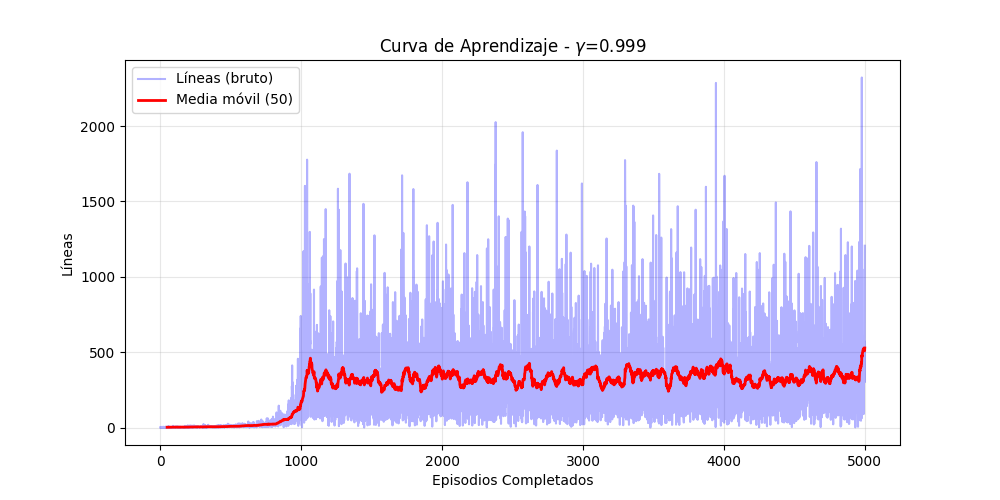
\includegraphics{figuras/curva_aprendizaje.png}}
\caption{Curva de aprendizaje obtenida para la mejor configuración del barrido: $\gamma=0.999$, $\alpha=0.001$ y $N_{\varepsilon}=1000$.}
\label{fig:curva_aprendizaje}
\end{figure}

La curva de aprendizaje permite respaldar empíricamente que el agente no solo ejecuta una política fija, sino que modifica progresivamente su comportamiento a partir de la experiencia obtenida durante los episodios de entrenamiento.

\subsection{Evolución de los pesos de la función de valor}

La Figura~\ref{fig:evolucion_pesos} presenta la evolución temporal de los pesos asociados a la aproximación lineal de la función de valor. Cada peso representa la importancia asignada por el agente a una característica del tablero, como altura, huecos, rugosidad, pozos o líneas eliminadas.

\begin{figure}
\centering
\resizebox{0.85\textwidth}{!}{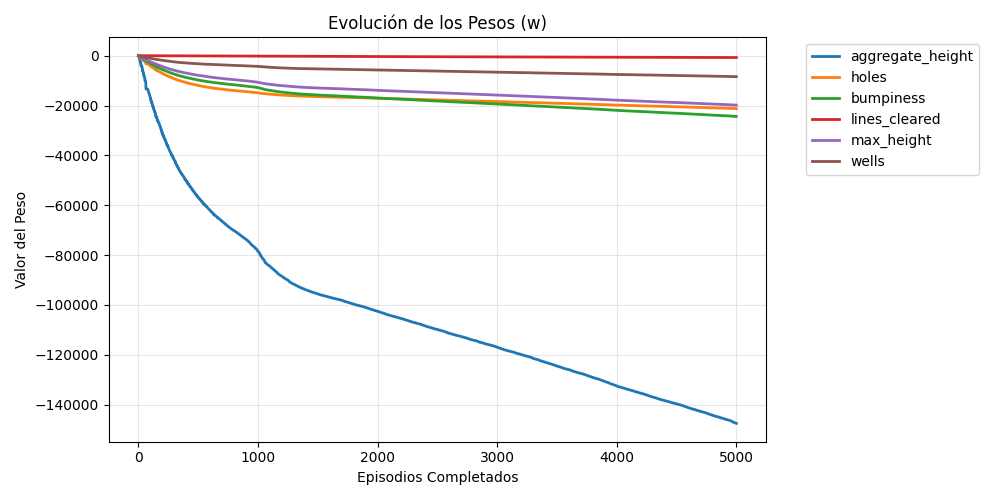
\includegraphics{figuras/evolucion_pesos.png}}
\caption{Evolución de los pesos de la función de valor para la mejor configuración de hiperparámetros.}
\label{fig:evolucion_pesos}
\end{figure}

La estabilización progresiva de los pesos constituye un indicio de que el proceso de aprendizaje converge hacia una valoración más consistente de los estados del tablero. En particular, la evolución de estos parámetros permite interpretar cómo el agente ajusta la importancia relativa de las características usadas para seleccionar acciones.

\subsection{Síntesis de resultados}

El barrido experimental permitió identificar una configuración capaz de eliminar en promedio $431.21$ líneas por partida antes de alcanzar el estado terminal. Este resultado confirma que la combinación de Aprendizaje por Refuerzo, aproximación lineal de funciones, representación mediante características y ajuste exhaustivo de hiperparámetros permite construir un agente competitivo para el entorno de Tetris considerado en este proyecto.
